\newpage
\section{Introdução} % Inicia a seção "Introdução"
\subsection{Contextualização}

\par A indústria é o setor da economia dedicado à produção de bens materiais, apoiado em trabalho humano, energia e equipamentos de alto valor agregado. Ao longo de sua evolução, sucessivos saltos tecnológicos redefiniram processos, produtos e formas de organização do trabalho, as chamadas "revoluções industriais" \cite{LASI_INDUSTRY_40}.

\par A Figura~\ref{fig:revolucoes_industriais} resume essa linha do tempo. Na primeira fase, destaca-se a mecanização da produção, na segunda, a difusão da energia elétrica e a produção em massa baseada no modelo Fordista e na terceira fase, a digitalização \cite{LASI_INDUSTRY_40}. Foi nessa fase que a introdução da tecnologia da informação, da automação e da eletrônica impulsionou o início da automação dos processos produtivos. Surgiram então os controladores lógicos programáveis (CLPs), os Controladores Numéricos Computadorizados (CNCs) e os robôs \cite{PISCHING2017}. Essas tecnologias tornaram-se essenciais para as indústrias que buscam maior eficiência e qualidade com menores custos e prazos. Sua adoção contribui diretamente para o aumento da produtividade \cite{BIGHETI2020}.


\begin{figure}[H]
    \centering
    \caption{Linha do Tempo das Revoluções Industriais}
    \centering
    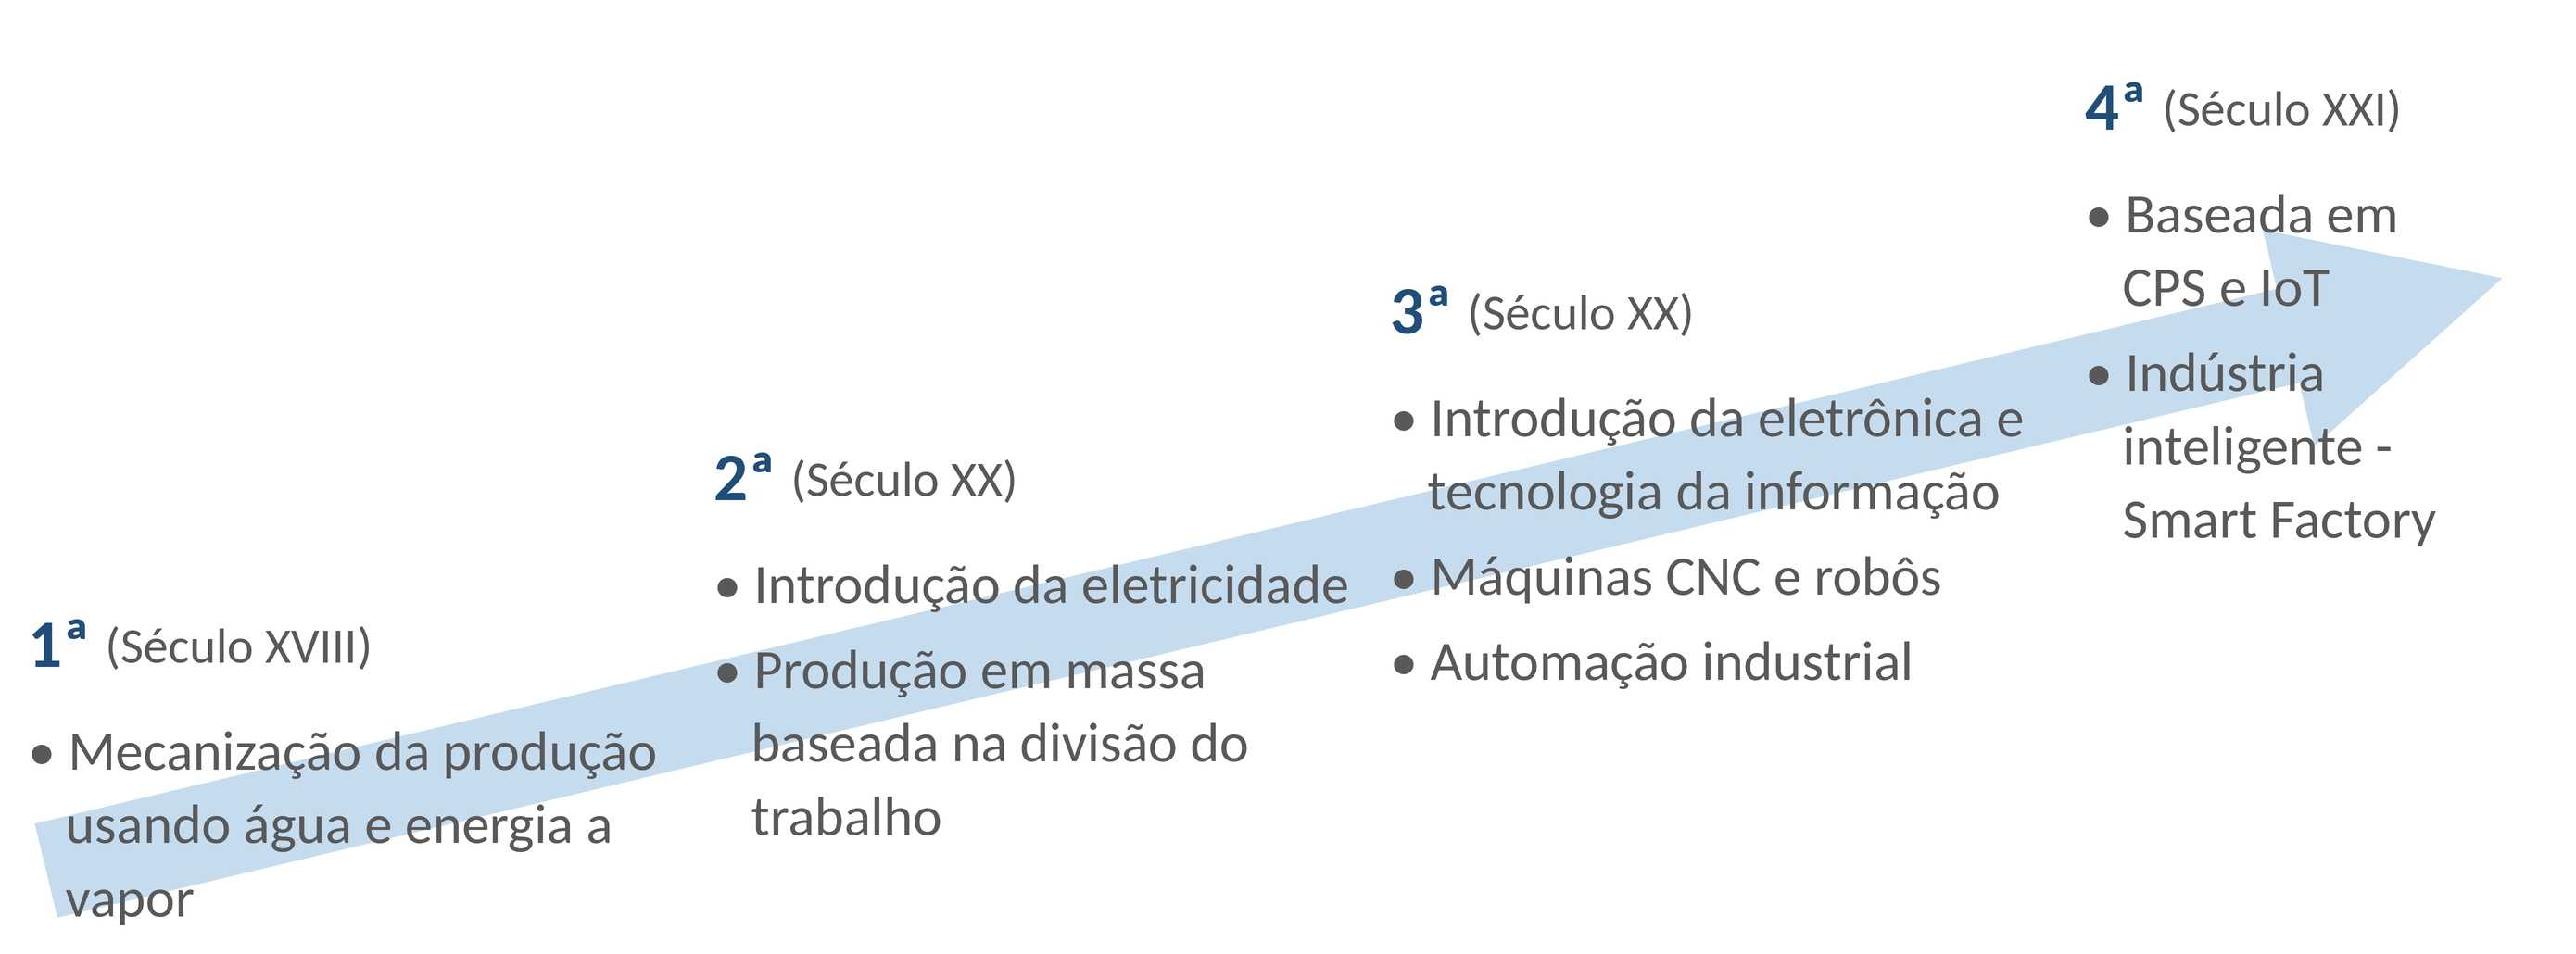
\includegraphics[width=0.9\textwidth]{Imagens/Introducao/Contextualizacao/evolucoes-industriais-nova.png}
    \centering
    \vspace{0.2cm} \\
    Fonte: Adaptado de \textcite{PISCHING2017}.
    \label{fig:revolucoes_industriais}
\end{figure}

\par Atualmente, vive-se a quarta fase, a chamada Indústria 4.0, baseada na indústria inteligente, na Internet das Coisas (\emph{Internet of Things}, IoT) e nos sistemas ciber-físicos (\emph{Cyber-Physical Systems}, CPS) \cite{BIGHETI2020}. Nesses sistemas, subsistemas computacionais cooperam entre si e permanecem integrados ao mundo físico e a seus processos, o que permite medir, controlar e analisar dados em tempo real por meio da rede, inclusive a Internet \cite{MONOSTORI2016_CPS_MANUFACTURING}.

\par A Figura~\ref{fig:piramide_automacao} organiza a automação na Indústria 4.0 em forma de pirâmide, distribuída em cinco níveis. No nível 0 está o processo físico de produção, com elementos como motores, bombas e tanques, no nível 1, o sensoriamento e a atuação, realizados por sensores, transmissores e válvulas. O nível 2 reúne o monitoramento, a supervisão e o controle, camada em que se encontram os controladores lógicos programáveis (CLPs), os sistemas supervisórios (SCADA) e as interfaces homem-máquina (IHM), responsáveis por acompanhar e comandar o processo em tempo real e por se comunicar com o nível 1 por protocolos seriais ou diretamente pelas entradas e saídas (I/O). O nível 3 corresponde às operações de manufatura e ao controle da produção, em que atuam os sistemas de execução da manufatura (\emph{Manufacturing Execution Systems}, MES). No topo, o nível 4 abrange o planejamento de negócios e a logística, em que se destacam os sistemas de gestão empresarial (\emph{Enterprise Resource Planning}, ERP) \cite{BIGHETI2020,COLOMBO2014_STATE_ART_AUTOMATION}.

\begin{figure}[H]
    \centering
    \caption{Pirâmide de Automação}
    \centering
    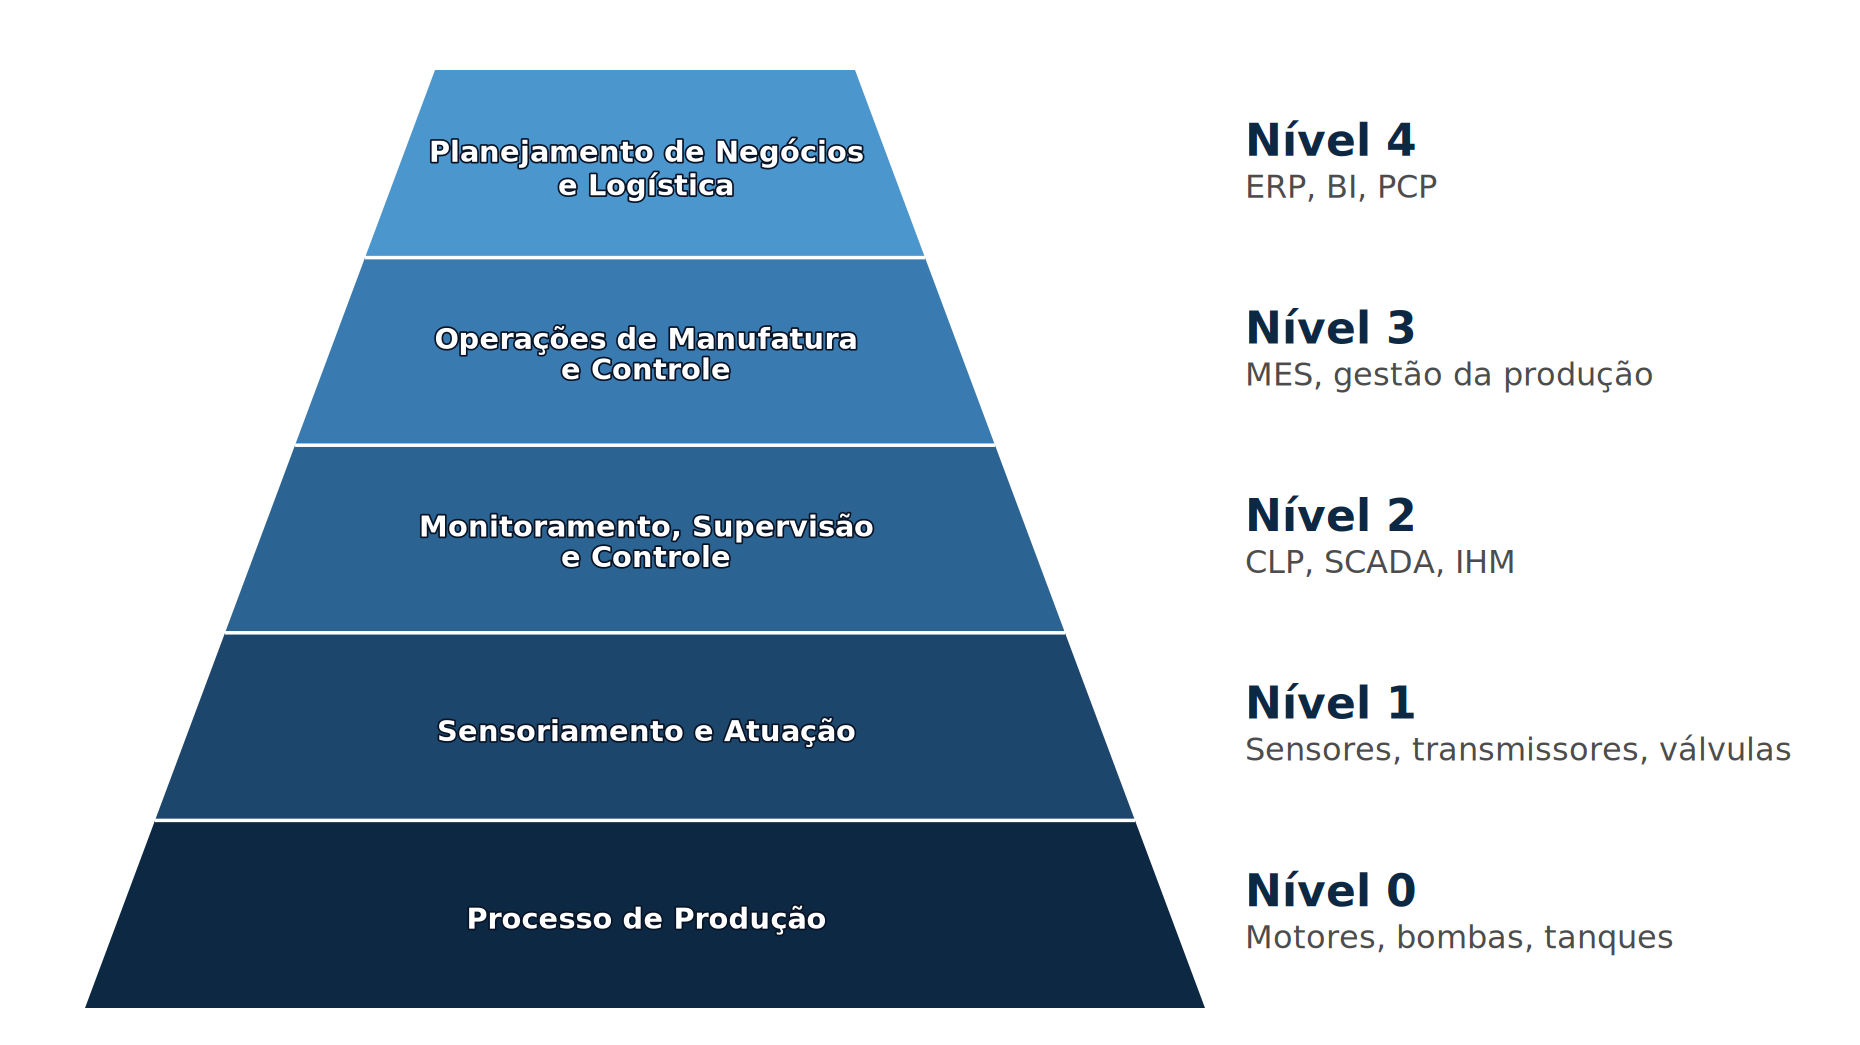
\includegraphics[width=0.9\textwidth]{Imagens/Introducao/Contextualizacao/piramide-automacao-nova.png}
    \centering
    \vspace{0.2cm} \\
    Fonte: Adaptado de \textcite{COLOMBO2014_STATE_ART_AUTOMATION}.
    \label{fig:piramide_automacao}
\end{figure}

\par Recentemente, as camadas de supervisão e de gestão, do nível 2 ao nível 4, ganharam mais notoriedade: ao digitalizar serviços antes restritos ao ambiente físico da planta, passou-se a ofertá-los sobre infraestrutura em nuvem e a compartilhá-los entre diferentes sistemas e usuários. Em geral, esses serviços seguem a arquitetura orientada a serviços (\emph{Service Oriented Architecture}, SOA), materializada por serviços Web (\emph{Web Services}, WS) \cite{COLOMBO2014_STATE_ART_AUTOMATION,AHMED2011_EFFICIENT_WEB_SCADA}. Esse movimento é sustentado pela própria natureza da Indústria 4.0, que se caracteriza pelo grande avanço dos protocolos de comunicação e de telemetria, pela popularização do desenvolvimento de software e pela interconexão inteligente de máquinas e sistemas \cite{LASI_INDUSTRY_40,PISCHING2017,BIGHETI2020}.

\par Tais avanços permitiram o monitoramento e a supervisão centralizada de processos complexos em tempo real, elevando o papel dos sistemas supervisórios de simples interfaces de operação para centrais estratégicas de análise de dados. Nesse cenário, este trabalho propõe o desenvolvimento de um sistema supervisório web orientado a serviços, que disponibiliza sobre infraestrutura em nuvem funcionalidades antes restritas ao ambiente físico da planta \cite{COLOMBO2014_STATE_ART_AUTOMATION}. Alinhada às tendências da Indústria 4.0 \cite{BIGHETI2020}, a proposta torna o monitoramento e a supervisão acessíveis e compartilháveis entre diferentes sistemas e usuários.